\documentclass[paper-main.tex]{subfiles}

\begin{document}

\begin{figure}
	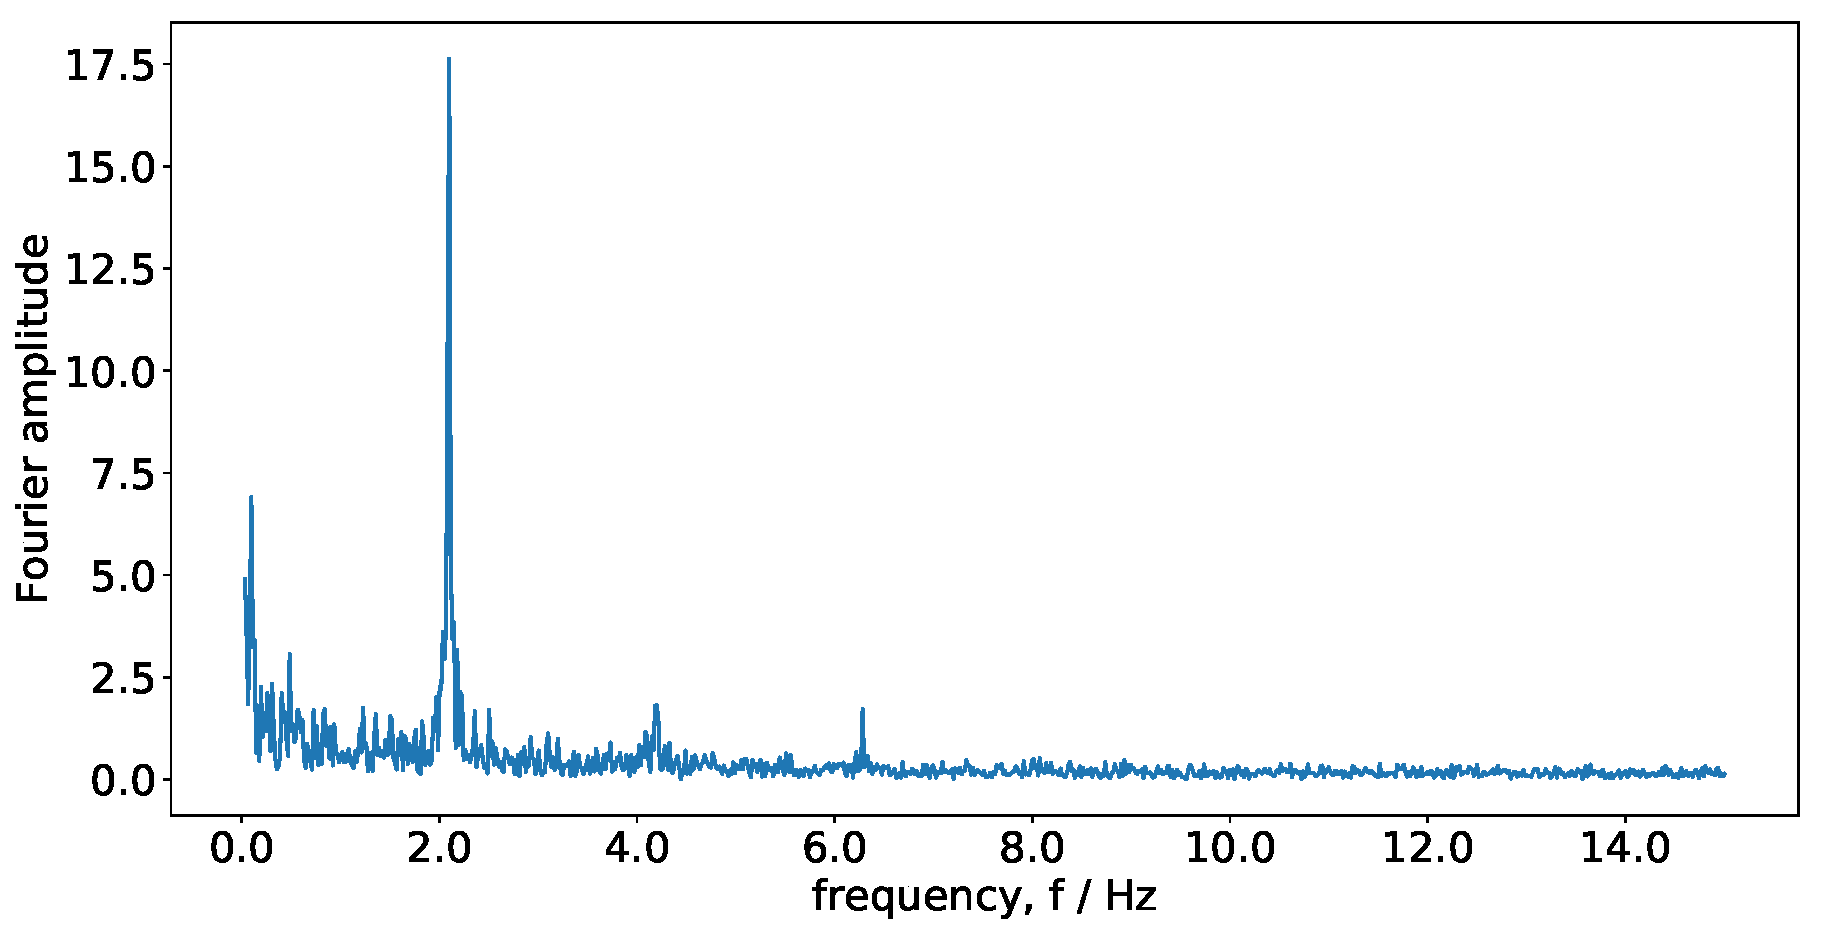
\includegraphics[width=.49\textwidth]{figures/webcam_expt_4_0209-cropped.pdf}
	\caption{\label{fig:webcam_spectrum}
Recovery of a tone at a constant frequency: Here we plot the Fourier amplitude of the intensity pattern against frequency.
The injected signal has a frequency of $2.09\,{\rm Hz}$, while the recovered signal peaks at $2.099\,{\rm Hz}$ and has a FWHM of $0.033\,{\rm Hz}$.
The plot also shows two harmonics at $4.19\,{\rm Hz}$ and $6.28\,{\rm Hz}$ with amplitudes $10.3 \%$ and $9.8 \%$ of the amplitude of the primary peak, respectively.
}	
\end{figure}

% rearranged as I found this section to switch between method and results too much, I've tried this order now: intro, webcam and data specifics, injection and results. 

Continuous-wave searches look for nearly monochromatic signals. In this section, we consider a simple sinusoidal tone at a single, constant frequency. %should be single constant frequency *signal*?

As described in Section~\ref{sec:ifo}, the audio signal is played through a speaker fixed to the back of M2. 
The intensity of the interference pattern is measured at a single point on the screen, indicated by the pink star in Fig~\ref{fig:interference_pattern}. 
The webcam records video in three colour channels; red, blue, and green. 
We use the green channel as an approximation of the total intensity produced by the monochromatic green laser.
The webcam samples at a rate of $30\, {\rm Hz}$, which limits the spectral content of observable signals to less than $15\,{\rm Hz}$, the Nyquist frequency. 


%The intensity of the interference pattern is measured at a single point on the screen using a commercial USB webcam (see Fig.~\ref{fig:ifo_schematic_webcam}). The webcam samples at a rate of $30\,{\rm Hz}$, which limits the spectral content of observable signals to below $15\,{\rm Hz}$, the Nyquist frequency. A tone with a frequency of $2.09\,{\rm Hz$} is played through the speaker for one minute and the interference pattern is recorded by the webcam.


%The pixel intensity in the green-channel of the video (the webcam records in three colour channels: red, blue, and green) is used to approximate the total intensity of the interference pattern. 
%This is because the laser emits monochromatic green light at $532\,{\rm nm}$.
A tone with a frequency of $2.09\,{\rm Hz}$ is played through the speaker for one minute. 
The amplitude of the Fourier transform of the recovered signal is shown in Fig.~\ref{fig:webcam_spectrum}. 
% removed 'strong' as what does strong mean here?
We measured a peak amplitude at $2.099\,{\rm Hz}$ with a full width half maximum (FWHM) of $0.033\,{\rm Hz}$. 
%Although this range doesn't contain our injected frequency, the error is not substantial and cannot be heard by the (untrained) human ear.
Two harmonics can also be seen at integer multiples of the peak frequency. 
The peaks at $4.19\,{\rm Hz}$ and $6.28\,{\rm Hz}$ have amplitudes of $0.103$ and $0.098$ as a fraction of the height of the main peak, respectively. They are likely due to the nonlinear response of the system discussed in Section~\ref{sec:ifo} and Appendix~\ref{app:intensity_derivation}.


In the following section, we use a hidden Markov model technique, commonly used in continuous wave searches, to recover a slowly wandering frequency signal.


\end{document}
